%%%%%%%%%%%%%%%%%%%%%%%%%%%%%%%%%%%%%%%%%
% Beamer Presentation
% LaTeX Template
% Version 1.0 (10/11/12)
%
% This template has been downloaded from:
% http://www.LaTeXTemplates.com
%
% License:
% CC BY-NC-SA 3.0 (http://creativecommons.org/licenses/by-nc-sa/3.0/)
%
%%%%%%%%%%%%%%%%%%%%%%%%%%%%%%%%%%%%%%%%%

%----------------------------------------------------------------------------------------
%	PACKAGES AND THEMES
%----------------------------------------------------------------------------------------

\documentclass{beamer}

\mode<presentation> {

% The Beamer class comes with a number of default slide themes
% which change the colors and layouts of slides. Below this is a list
% of all the themes, uncomment each in turn to see what they look like.

%\usetheme{default}
%\usetheme{AnnArbor}
%\usetheme{Antibes}
%\usetheme{Bergen}
%\usetheme{Berkeley}
%\usetheme{Berlin}
%\usetheme{Boadilla}
%\usetheme{CambridgeUS}
%\usetheme{Copenhagen}
%\usetheme{Darmstadt}
%\usetheme{Dresden}
%\usetheme{Frankfurt}
%\usetheme{Goettingen}
%\usetheme{Hannover}
%\usetheme{Ilmenau}
%\usetheme{JuanLesPins}
%\usetheme{Luebeck}
\usetheme{Madrid}
%\usetheme{Malmoe}
%\usetheme{Marburg}
%\usetheme{Montpellier}
%\usetheme{PaloAlto}
%\usetheme{Pittsburgh}
%\usetheme{Rochester}
%\usetheme{Singapore}
%\usetheme{Szeged}
%\usetheme{Warsaw}

% As well as themes, the Beamer class has a number of color themes
% for any slide theme. Uncomment each of these in turn to see how it
% changes the colors of your current slide theme.

%\usecolortheme{albatross}
%\usecolortheme{beaver}
%\usecolortheme{beetle}
%\usecolortheme{crane}
%\usecolortheme{dolphin}
%\usecolortheme{dove}
%\usecolortheme{fly}
%\usecolortheme{lily}
%\usecolortheme{orchid}
%\usecolortheme{rose}
%\usecolortheme{seagull}
%\usecolortheme{seahorse}
%\usecolortheme{whale}
%\usecolortheme{wolverine}

%\setbeamertemplate{footline} % To remove the footer line in all slides uncomment this line
%\setbeamertemplate{footline}[page number] % To replace the footer line in all slides with a simple slide count uncomment this line

%\setbeamertemplate{navigation symbols}{} % To remove the navigation symbols from the bottom of all slides uncomment this line
}

\usepackage{graphicx} % Allows including images
\DeclareGraphicsExtensions{.pdf,.png,.jpg}
\usepackage{booktabs} % Allows the use of \toprule, \midrule and \bottomrule in tables
\usepackage[skip = 2pt, font=scriptsize]{caption}
\usepackage{subfigure}

%----------------------------------------------------------------------------------------
%	TITLE PAGE
%----------------------------------------------------------------------------------------

\title[Antineutrons]{Discovery of the W-Boson} % The short title appears at the bottom of every slide, the full title is only on the title page

\author{Oliver Dahme} % Your name
\institute[UZH] % Your institution as it will appear on the bottom of every slide, may be shorthand to save space
{
University of Zurich \\ % Your institution for the title page
\medskip
\textit{o.dahme@cern.ch} % Your email address
}
\date{\today} % Date, can be changed to a custom date

\begin{document}

\begin{frame}
\titlepage % Print the title page as the first slide
\end{frame}

% \begin{frame}
% \frametitle{Overview} % Table of contents slide, comment this block out to remove it
% \tableofcontents % Throughout your presentation, if you choose to use \section{} and \subsection{} commands, these will automatically be printed on this slide as an overview of your presentation
% \end{frame}

%----------------------------------------------------------------------------------------
%	PRESENTATION SLIDES
%----------------------------------------------------------------------------------------

%------------------------------------------------
\section{Introduction} % Sections can be created in order to organize your presentation into discrete blocks, all sections and subsections are automatically printed in the table of contents as an overview of the talk
%------------------------------------------------

\begin{frame}
\frametitle{Postulate}
\begin{itemize}
  \item $q \rightarrow q$ + $e^\pm$ + $\nu$ mediated by 2 massive bosons
  \item should result in enhancement of: $q$ + $\bar{q} \rightarrow e^\pm$ + $\nu$ cross section
  \item $M_W$ predicted at $(82 \pm 2.4)$ GeV/$c^2$
\end{itemize}
\end{frame}
%------------------------------------------------

\begin{frame}
\frametitle{Detector}
\begin{itemize}
  \item $(7 \cdot 3.5 \cdot 3.5) m^3$ transverse dipole magnet with 0.7 T
  \item cylindric drift chamber, 3.5 m long and diameter of 2.3 m arround the interaction point
  \item yields a bubble-chamber picture of each $p \bar{p}$ interaction
\end{itemize}
\end{frame}

%------------------------------------------------

\begin{frame}
\frametitle{Calorimetry}
\begin{figure}
  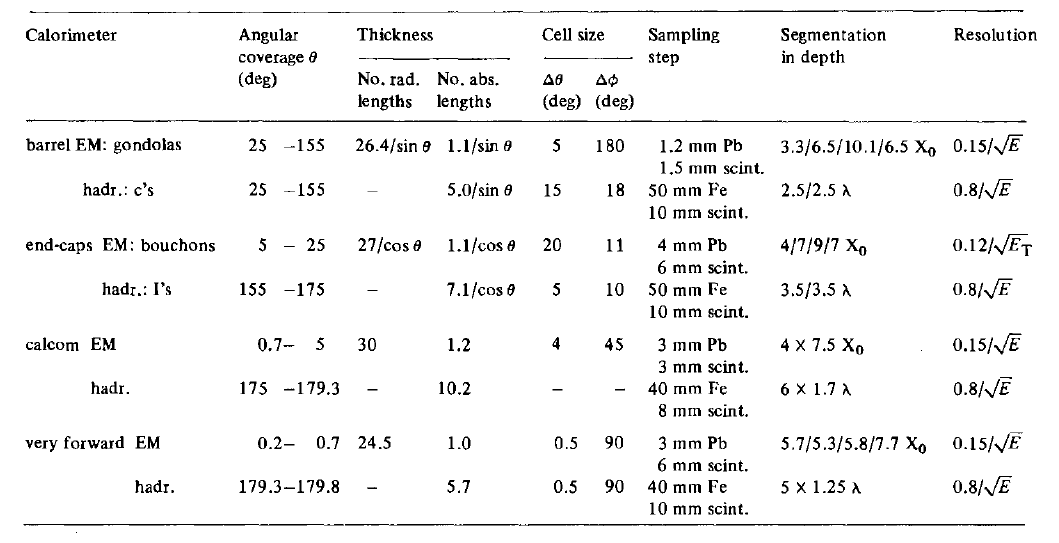
\includegraphics[width=1.0\textwidth]{calorimetry}
  \caption{Calorimetry of the Experiment}
  \label{fig:calorimetry}
\end{figure}
\end{frame}

\begin{frame}
\frametitle{Detection}
\begin{itemize}
  \item Electrons leave no track in the hadronic calorimeter (98\%)
  \item Neutrinos by missing energy, due to a hermetic calorimetry down to $0.2^o$
  \item muons by muon chamber arround the experiment
\end{itemize}
\end{frame}

\begin{frame}
\frametitle{Data}
\begin{itemize}
  \item Data-taking in a 30-day period during Nov and Dez 1982
  \item minimum transvers energy of 10 GeV
  \item 3 triggers:
  \begin{enumerate}
    \item jet trigger with 15 GeV in a localized region
    \item global transvers energy trigger with $>$ 40 GeV
    \item muon trigger at least one penetrating track to the diamond (vertex)
  \end{enumerate}
  \item electrons have to be isolated
  \item energetic neutrinos required
\end{itemize}
\end{frame}

\begin{frame}
\frametitle{Most important events}
\begin{figure}
  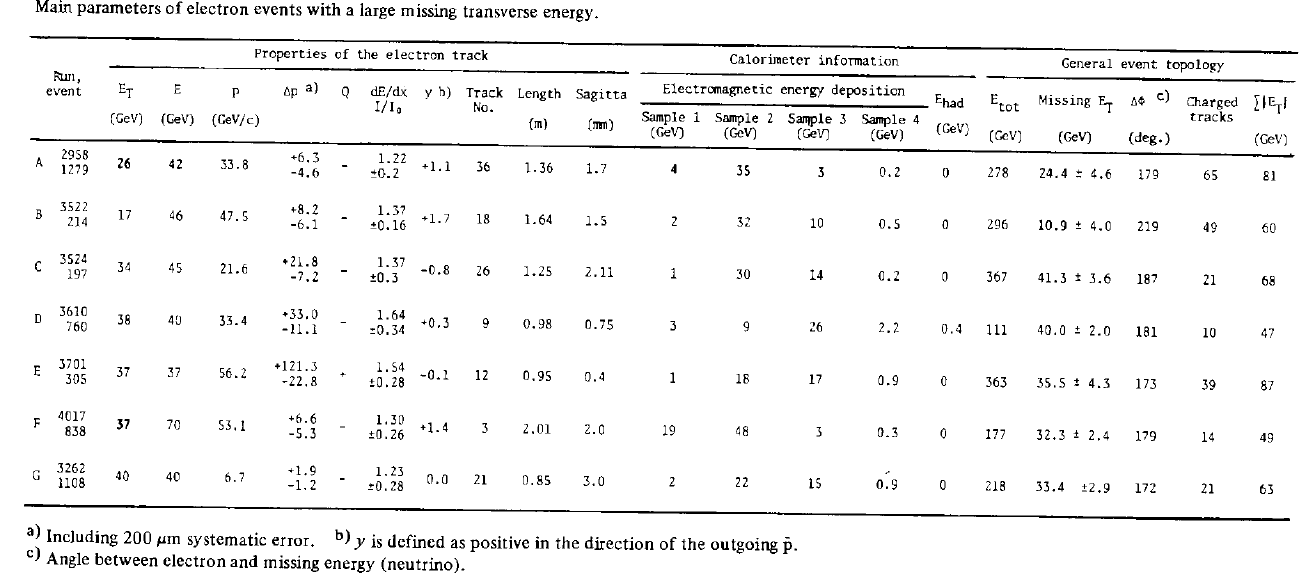
\includegraphics[width=1.0\textwidth]{events}
  \caption{The last 7 events after triggering and filtering}
\end{figure}
\end{frame}

\begin{frame}
\frametitle{digital events}
\begin{figure}
  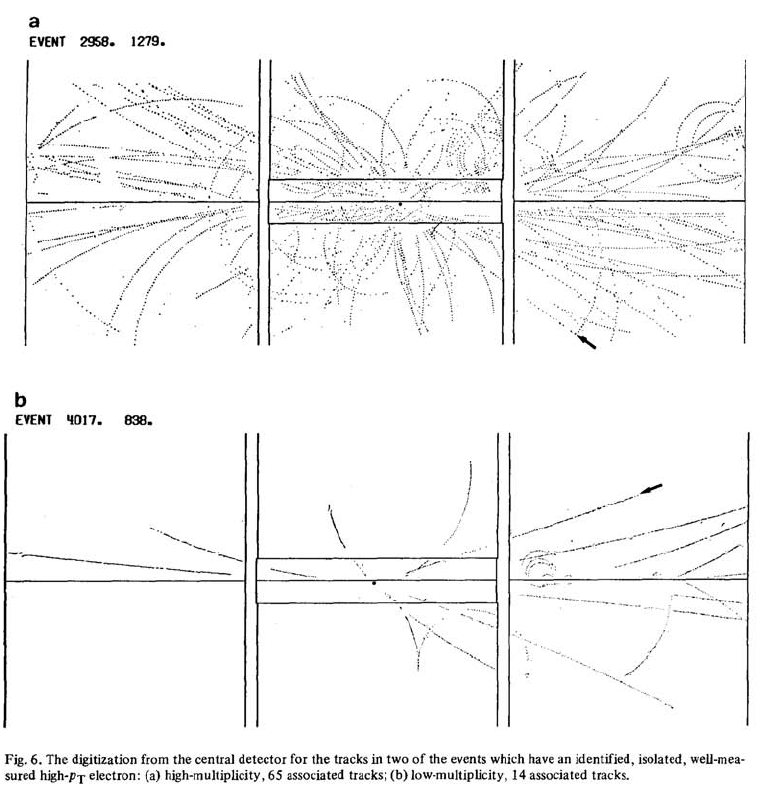
\includegraphics[width=0.5\textwidth]{digital_event}
  %\caption{}
\end{figure}
\end{frame}


\section{Results}
%------------------------------------------------
\begin{frame}
  \frametitle{relevant events}
  \begin{figure}
    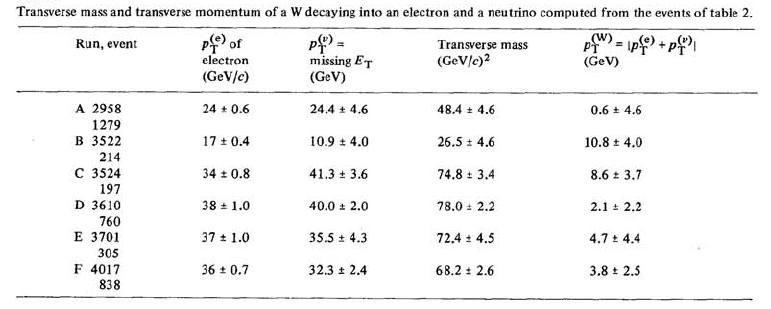
\includegraphics[width=1.0\textwidth]{events2}
    \caption{candidates for W decay}
  \end{figure}
\end{frame}

\begin{frame}
  \frametitle{Analysis}
  \begin{figure}
    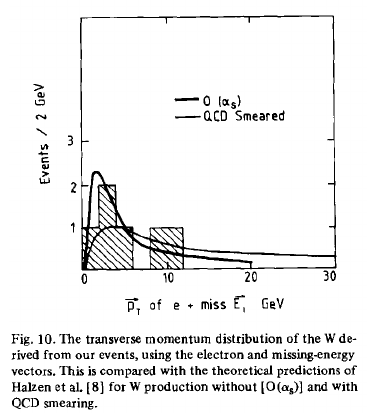
\includegraphics[width=0.45\textwidth]{result}
    %\caption{}
  \end{figure}
  \begin{itemize}
    \item The fit lead to a $m_W = (81 \pm 5)$ GeV/$c^2$
    \item theory predicted $m_W = (74 \pm 4)$ GeV/$c^2$
    \item The result is in excellent agreement with the expactations
  \end{itemize}
\end{frame}

%------------------------------------------------
\begin{frame}
\frametitle{Questions?}
\end{frame}

%------------------------------------------------

%------------------------------------------------

%----------------------------------------------------------------------------------------

\end{document}
